% ----------------------------------------------------------
% Introdução (exemplo de capítulo sem numeração, mas presente no Sumário)
% ----------------------------------------------------------
\chapter[Introdução]{Introdução}
%\addcontentsline{toc}{chapter}{Introdução}
% ----------------------------------------------------------
\par O Estado de São Paulo sofreu com problemas da crise hídrica, decorrente pelo fato do consumo excessivo e uso inconsciente da água  dentre outros fatores. Esse problema afetou também a região do Vale do Paraíba, como pode ser observado no relatório da ANA \cite{ana1}, onde o Sistema Hidráulico Paraíba do Sul observou uma redução acelerada dos níveis das represas e esteve operando meses em estado de alerta. Assim foi tomada atitude mais emergenciais como intensificar as manobras de redução de pressão e também o bombeamento do volume morto, com águas mais sujas que ficam no fundo das represas, e também pedir para população se conscientizar e racionar o consumo de água.

 
\begin{figure}[h]
	\caption{\textbf{Volume Útil dos Reservatórios do Sistema Hidráulico Paraíba do Sul}}
	\centering
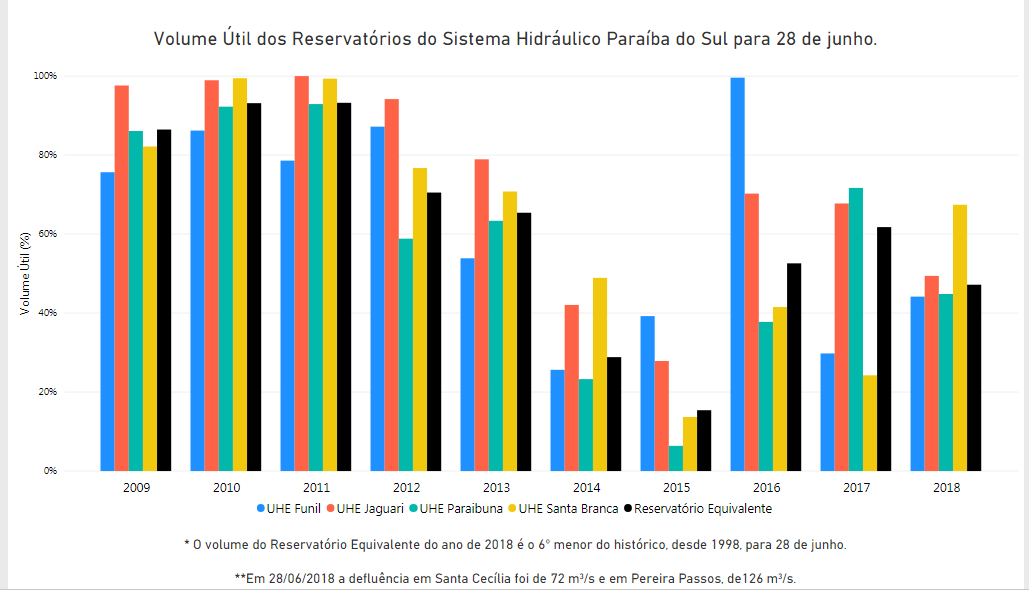
\includegraphics[width=\textwidth,height=\textheight ,keepaspectratio]{figuras/situacaoreservatoriosvaleparaiba}
    \label{fig:ana}	
	\fonte{Adaptada pelo autor, de \citeonline{ana1}}
\end{figure}



% ######## init table ########
\begin{table}[ht]
\caption{ \textbf{Dados dos Volumes Útil dos Reservatórios do Sistema Hidráulico Paraíba do Sul}}
\centering
\begin{tabular}{|c|c|c|c|c|c|}
\hline
\rowcolor[HTML]{80C397} 
\textbf{ANO}                          & \textbf{\begin{tabular}[c]{@{}c@{}}UHE \\ Funil\end{tabular}} & \textbf{\begin{tabular}[c]{@{}c@{}}UHE\\  Jaguari\end{tabular}} & \textbf{\begin{tabular}[c]{@{}c@{}}UHE\\  Paraibuna\end{tabular}} & \textbf{\begin{tabular}[c]{@{}c@{}}UHE\\  Santa Branca\end{tabular}} & \textbf{\begin{tabular}[c]{@{}c@{}}Reservatório \\ Equivalente\end{tabular}} \\ \hline
\textbf{2009}                         & \textbf{75,66\%}                                              & \textbf{97,62\%}                                                & \textbf{86,10\%}                                                  & \textbf{82,18\%}                                                     & \textbf{86,47\%}                                                             \\ \hline
\rowcolor[HTML]{80C397} 
\textbf{2010}                         & \textbf{86,21\%}                                              & \textbf{98,95\%}                                                & \textbf{92,26\%}                                                  & \textbf{99,45\%}                                                     & \textbf{93,15\%}                                                             \\ \hline
\textbf{2011}                         & \textbf{78,60\%}                                              & \textbf{103,11\%}                                               & \textbf{92,92\%}                                                  & \textbf{99,36\%}                                                     & \textbf{93,24\%}                                                             \\ \hline
\rowcolor[HTML]{80C397} 
\textbf{2012}                         & \textbf{87,20\%}                                              & \textbf{94,18\%}                                                & \textbf{58,84\%}                                                  & \textbf{76,72\%}                                                     & \textbf{70,51\%}                                                             \\ \hline
\textbf{2013}                         & \textbf{53,87\%}                                              & \textbf{78,93\%}                                                & \textbf{63,36\%}                                                  & \textbf{70,78\%}                                                     & \textbf{65,40\%}                                                             \\ \hline
\rowcolor[HTML]{80C397} 
\textbf{2014}                         & \textbf{25,63\%}                                              & \textbf{42,06\%}                                                & \textbf{23,27\%}                                                  & \textbf{48,92\%}                                                     & \textbf{28,84\%}                                                             \\ \hline
\cellcolor[HTML]{FFFFFF}\textbf{2015} & \textbf{39,23\%}                                              & \textbf{27,87\%}                                                & \textbf{63,80\%}                                                  & \textbf{13,69\%}                                                     & \textbf{15,40\%}                                                             \\ \hline
\rowcolor[HTML]{80C397} 
\textbf{2016}                         & \textbf{99,60\%}                                              & \textbf{70,25\%}                                                & \textbf{37,77\%}                                                  & \textbf{41,53\%}                                                     & \textbf{52,59\%}                                                             \\ \hline
\textbf{2017}                         & \textbf{29,78\%}                                              & \textbf{67,75\%}                                                & \textbf{71,69\%}                                                  & \textbf{24,24\%}                                                     & \textbf{61,77\%}                                                             \\ \hline
\rowcolor[HTML]{80C397} 
\textbf{2018}                         & \textbf{44,16\%}                                              & \textbf{49,42\%}                                                & \textbf{44,84\%}                                                  & \textbf{67,43\%}                                                     & \textbf{47,18\%}                                                             

\end{tabular}
\label{table:table_ana}
\fonte{Adaptada pelo autor, de \citeonline{ana1}}
\end{table}
  	
 
\par O problema pode ser observado na figura \ref{fig:ana} e na tabela \ref{table:table_ana}, visualizando os níveis dos reservatórios que oscilam, isso é alarmante. Visto isso, a empresa TecSUS Tecnologias para a Sustentabilidade desenvolveu tecnologias que ajudam na economia dos recursos escassos do planeta e aumentam a eficiência de processos e produtos. Com produto TecHydro, monitoramento e controle remoto de hidrômetros, podendo ser para uso doméstico, comercial e industrial. A coleta de dados de consumo de água em intervalos pré-programados (entre 1 minuto e 24 horas). Com os dados obtidos, a empresa analisa o consumo e gera um relatório.

\par 


\section{Motivação}
\par Foi escolhido esse tema para realizar um estudo no consumo de água para investigação de detecção possível excesso e vazamento em residências e empresas, com aplicação de \emph{data mining}, visando economia no consumo de água.
\section{Objetivos}
\par As subseções a seguir apresentam os objetivos deste trabalho.
\subsection{ Objetivo Geral}
\par Este trabalho de graduação tem por objetivo desenvolver um estudo para se identificar possíveis desperdícios de água em residências e empresas, com aplicação de \emph{data mining}, visando economia no consumo de água.
\subsection{Objetivo Específico}
\par Para a realização deste  foram estabelecidos os objetivos específicos:
\begin{itemize}
	\item Realizar a captação de dados no estilo xlsx;
	\item Fazer a mineração dos dados coletados;
	\item Fazer a análise dos dados coletados;
	\item Fazer a plotagem dos dados coletados em gráficos;
\end{itemize}
